\def \sectionauthors {Dennis Köb}
\subsection{Anforderungen}
Das Ziel der Fahrzeugerkennung ist es Fahrzeuge auf mehrere Parklücken eines Parkplatzes zu erkennen. Die daraus 
gewonnen Zustände sollen an das Webinterface übermittelt und an den jeweilige Parklücken über LEDs ausgegeben werden. 
\subsection{Vorstudie}

\subsection{Erkennung von Metallen über Spulen}
Grundsätzlich werden in der Realität häufig Spulen verwendet, welche unter dem Asphalt verbaut sind, um darüberliegende
Fahrzeuge zu detektieren. Als Messprinzip wird die Änderung des magnetischen Widerstands $R_{m}$ bei konstanter magnetischer Spannung $U_{m}$ und
daraus resultierende magnetischen Fluss $\phi$
Es gelten für diese Größen der folgende Zusammenhänge:

\begin{equation} \label{eq:phi}
    \Phi = \frac{U_{m}}{R_{m}}
\end{equation}

Wobei \\
$\Phi$ = magnetischer Fluss \\
$R_{m}$ = magnetischer Widerstand \\
$U_{m}$ = magnetische Spannung
\pagebreak

Der magnetische Widerstand lässt sich wiederum durch die Eigneschaften der Spule bestimmen. Die Formel hierfür lautet:

\begin{equation} \label{eq:Rm}
    R_{m} = \frac{N \cdot (2a + 2b)}{\mu_{0} \cdot \mu_{r} \cdot A} 
\end{equation}


Wobei \\
\begin{equation} \label{eq:A}
    A = a \cdot b
\end{equation}
$N$ = Anzahl der Windungen der Spule \\
$a$ = Breite der Spule in m \\
$b$ = Länge der Spule in m\\
$\mu_{0}$ = \SI[per-mode = symbol]{1.2566e-6}{\newton\per\ampere\squared} = magnetische Feldkonstante \\
$\mu_{r}$ = relative Permeabilität  \\
$A$ = Fläche der Spule

Bis auf die relative Permeabilität sind alle alle anderen Variablen konstant. Daraus lässt sich schlussfolgern, dass der magnetische
Fluss $\Phi$ anhand der Gleichung \ref{eq:phi} und \ref{eq:Rm} proportional zur relativen Permeabilität ist. 

\begin{equation} \label{iq:phi}
    \Phi \propto \mu_{r}
\end{equation}
Der Fluss $\Phi$ hängt somit auch von den Materialien ab durch die er fließt. In der nächsten Abbildung kann man erkennen,
wie ein Fahrzeug über eine im Boden installierte Spule den magnetischen Fluss $\Phi$ und somit die magnetische Flussdichte $B$
beeinflussen kann. 

\begin{figure}[H]
    \centering
    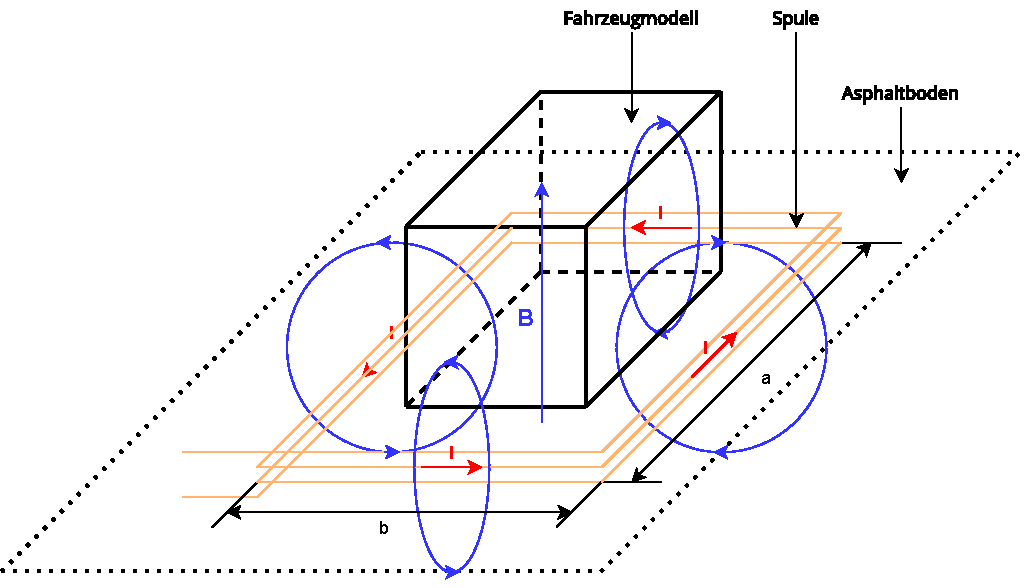
\includegraphics[width=1\linewidth]{fahrzeugerkennung/Spuleninstallation.pdf}
    \caption{Installation der Spule}
  \end{figure}
Um diese Größen auslesbar zu machen, müssen diese magnetischen bei einer direkten Messung in elektrische Größen umgewandelt
werden.
Hierfür gelten folgende Zusammenhänge:

\begin{equation} \label{eq:L_phi}
    L = \frac{N \cdot \Phi}{I} = \frac{\Psi}{I} 
\end{equation}
Wobei \\
$L$ = Induktivität der Spule \\
$I$ = Strom der durch die Spule fließt \\
$N$ = Anzahl der Windungen der Spule \\
$\Psi$ = Verkettete Fluss

\pagebreak
\begin{equation} \label{eq:L_i}
    u(t) = L \cdot \frac{di(t)}{dt}
\end{equation}

Wobei \\
$L$ = Induktivität der Spule \\
$i(t)$ = Strom der durch die Spule fließt zum Zeitpunkt t \\
$u(t)$ = Spannung die an der Spule anliegt zum Zeitpunkt t \\
$t$ = Zeit in s \\
So lässt sich bei Bekanntheit von Strom und Spannung auf die Induktivität und mit der Gleichung \ref{eq:L_phi} 
und mit den Zusammenhang \ref{iq:phi} auf die magnetischen Eigenschaften des Materials rückschließen. 
Diese Art der Detektion bietet viele praktische Vorteile.

\begin{itemize}
    \item \textbf{Größerer Messbereich} \\
    Im Vergleich zu anderen Detektionsmethoden wie einer Leichtschranke kann man einen größeren Bereich durch die Wirkfläche
    der Spule abdecken. So lassen sich auch kleinere Kraftfahrzeuge wie Motorräder oder Mopeds besser erkennen.
    \item \textbf{Schutz vor Umweltfaktoren} \\
    Durch den Verbau im Boden ist die Messeinrichtung vor Umwelteinflüssen wie Regen, Frost, hohen beziehungsweise
    niedrigen Temperaturen und Korrosion besser geschütz. Dies verringert auch den Einfluss dieser Störfaktoren auf die Eigenschaften
    Spule und somit auf die daraus resultierenden Messergebnisse.
    \item \textbf{Ausschließung von Materialien} \\
    Alle nicht metallische Stoffe werden von diesem Messprinzip nicht wahrgenommen. So können Verschmutzungen wie Blätter und Staub, welche
    visuelle Sensoren stören können, die Detektion nicht behindern.
    
\end{itemize}
\subsubsection{Messung ferromagnetischer Metalle}
Um diese Dtektionsverfahren zu verstehen muss zuerst der Zusammenhang zwischen Induktivität und relativer Permeabilität verstanden werden.
Aus den Gleichungen \ref{eq:Rm}, \ref{eq:phi} und \ref{eq:L_phi} kann die folgende Proportionalität ermittelt werden:
\begin{equation} \label{iq:L_mu}
    L \propto \mu_{r}
\end{equation}
Bei ferromagnetischen Stoffen wie Eisen ist die relative Permeabilität sehr viel größer als 1. Wenn nun ein Auto oder 
eine anderes Vehikel sehr viel Eisen beinhaltet wirkt sich die dies steigernd auf die Induktivität der Spule aus. Die folgenden
Verfahren nutzen dieses Prinzip um die Belegung einer Parklücke zu bestimmen.

\paragraph{RL-Oszillator mit Timer Baustein}\mbox{}\\
Bei diesem Messverfahren wird die Änderung der Induktivität $L$ über die Änderung einer Stromladekurve über einen Widerstand
$R$ ermittelt. Eine Simulation in LTSPice mit folgendem Schaltbild kann die Auswirkung auf eine Ladekurve bei gleicher Spannung
und gleichem Widerstand gut darstellen.
\begin{figure}[H]
    \centering
    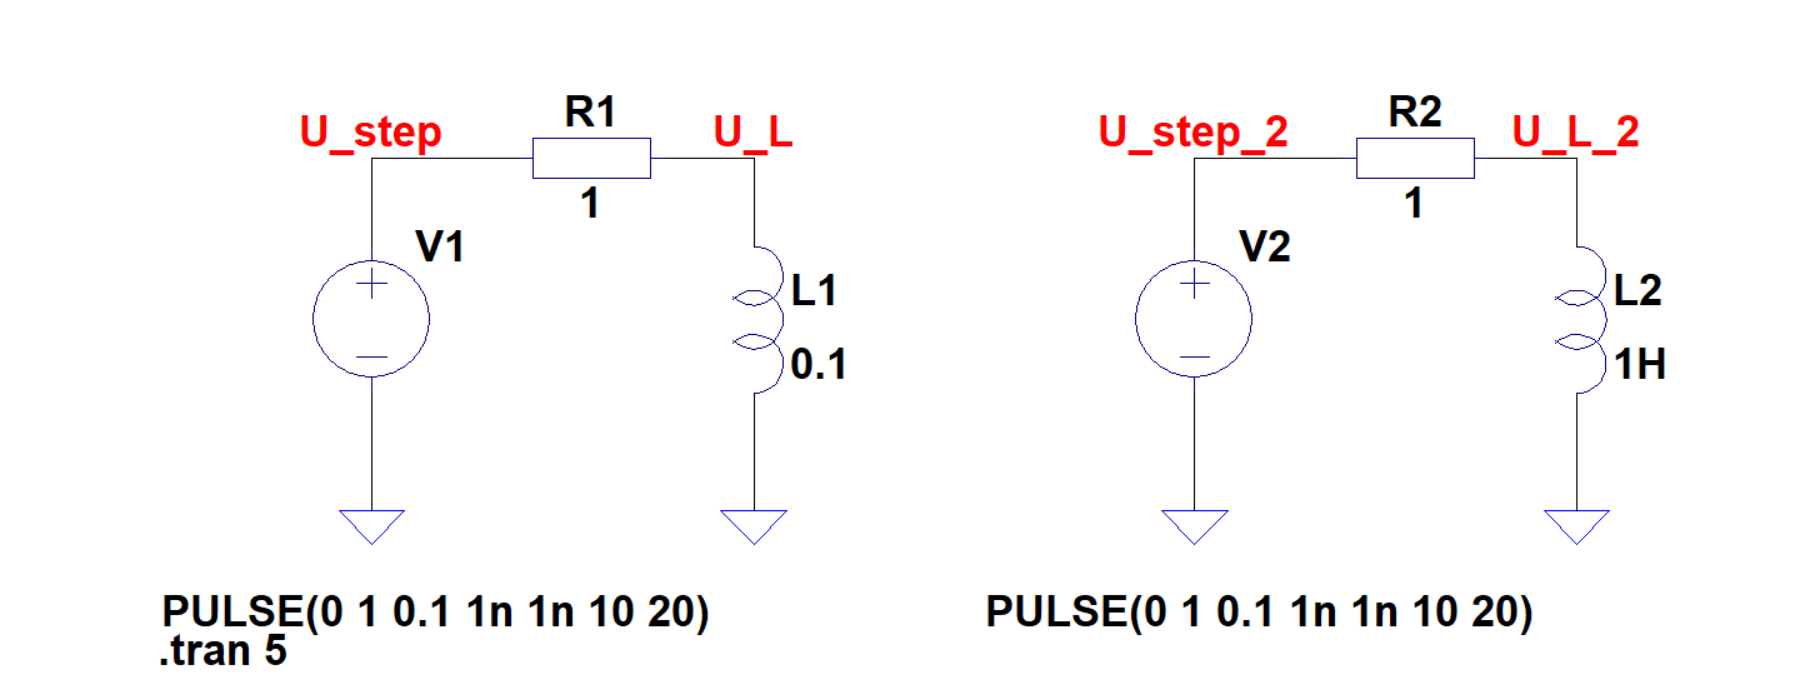
\includegraphics[width=1\linewidth]{fahrzeugerkennung/Ladekurven.png}
    \caption{LTSPice Blockbild zweier RL-Glieder}
\end{figure}
\pagebreak
Die daraus Resultierende Simulation im Zeitbereich ergibt folgendes Ergebnis:
hmm

\begin{figure}[H]
    \centering
    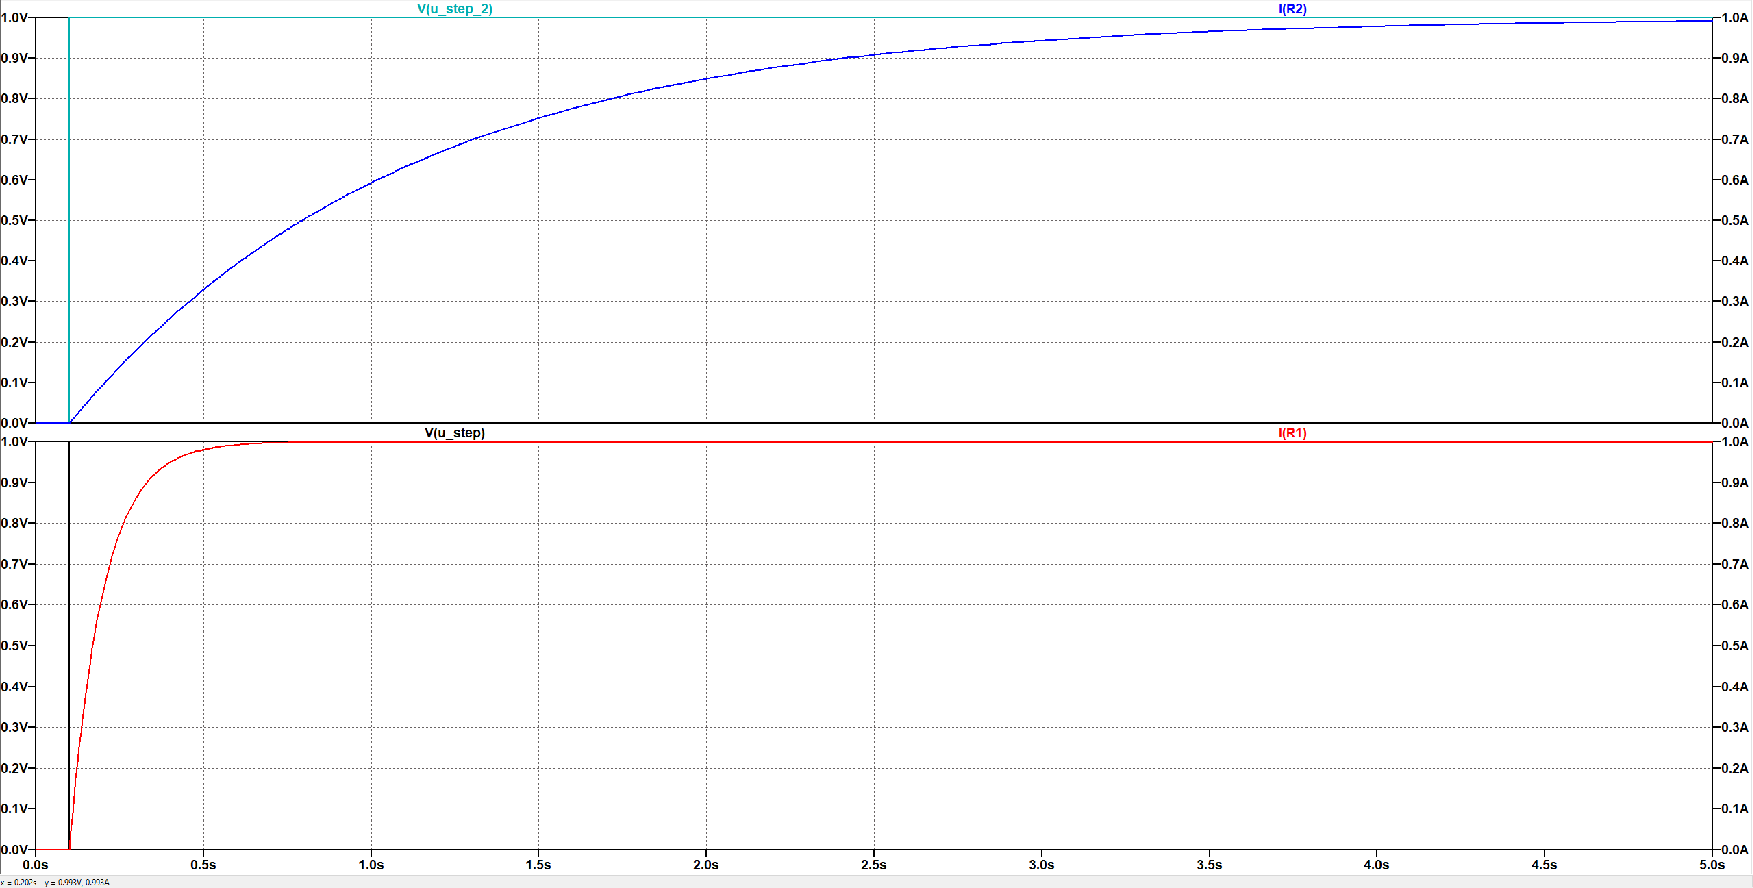
\includegraphics[width=1\linewidth]{fahrzeugerkennung/Ladekurven_ZB.png}
    \caption{Stromkurven zweier RL-Glieder}
\end{figure}

Es ist aus der letzten Abbildung erkennbar, dass sich eine größere Induktivität verlangsamend auf die Zunahme des Stromes auswirkt. Für Einschaltvorgänge kann diese Stromkurve
für RL-Glieder folgendermaßen beschrieben werden.

\begin{equation} \label{eq:i_L}
    i(t) = \frac{U_{0}}{R} \cdot (1 - e^{-\frac{t}{\tau}})
\end{equation}

\begin{equation} \label{eq:tau_RL}
    \tau = \frac{L}{R}
\end{equation} 

Wobei \\
$i(t)$ = Strom der durch die Spule fließt zum Zeitpunkt t \\
$L$ = Induktivität der Spule in H\\
$R$ = Widerstand in $\Omega$ \\
$U_0$ = Spannung die nach dem einschalten anliegt in V\\
$t$ = Zeit in s \\
$\tau$ = Zeitkonstante in $\frac{1}{s}$\\

Timer Bausteine wie der NE555 nutzen diese solche Verlaufskurven wenn sie als astabile Kippstufe konfiguriert sind.
Es gibt einen Eingang dieses Baustein meist CV für Control Voltage der die Spannung überwacht. Überschreitet diese Spannung zweit drittel
der Betriebsspannung schaltet er einen weiteren Pin, meist DIS für Discharge, auf 0V beziehungsweise auf Masse. Unterschreitet jedoch 
die Spannung am CV Pin ein drittel der Betriebsspannung so wird der DIS Pin auf Betriebsspannung geschalten. Diese beiden Pins 
sind über RC- oder RL- Glieder verbunden. Es entsteht somit ein Oszillator, welcher die Spannung am DIS Pin anhebt und absenkt.
Der NE555 kann dieses Signal über einen internen Komparator in ein Rechtecksignal umwandeln, welches besser von Mikrokontrollern ausgelesen
werden kann. Der Mikrokontroller kann so die Anzahl der ein einkommenden Takte über einen gewissen Zeitraum zählen und daraus eine Oszillatorfrequenz errechnen.
Die Zeitsignale lassen sich in LTSPice mit dem NE555 als Timer-Baustein simulieren.

\begin{figure}[H]
    \centering
    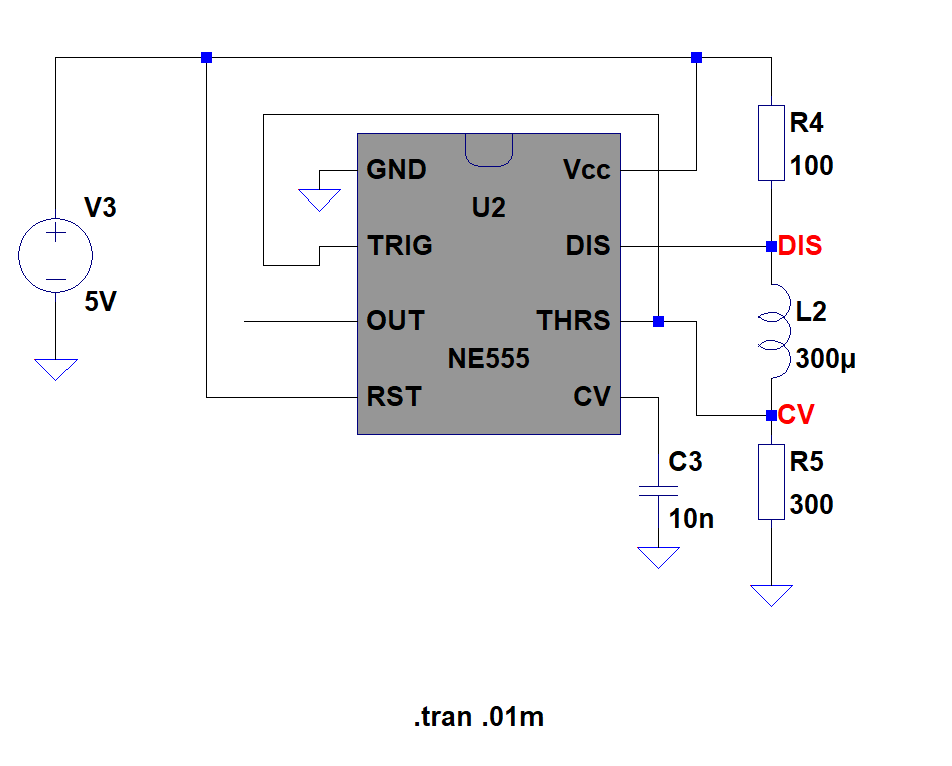
\includegraphics[width=0.6\linewidth]{fahrzeugerkennung/RL_Oszillator.png}
    \caption{RL-Oszillator mit NE555}
\end{figure}

\begin{figure}[H]
    \centering
    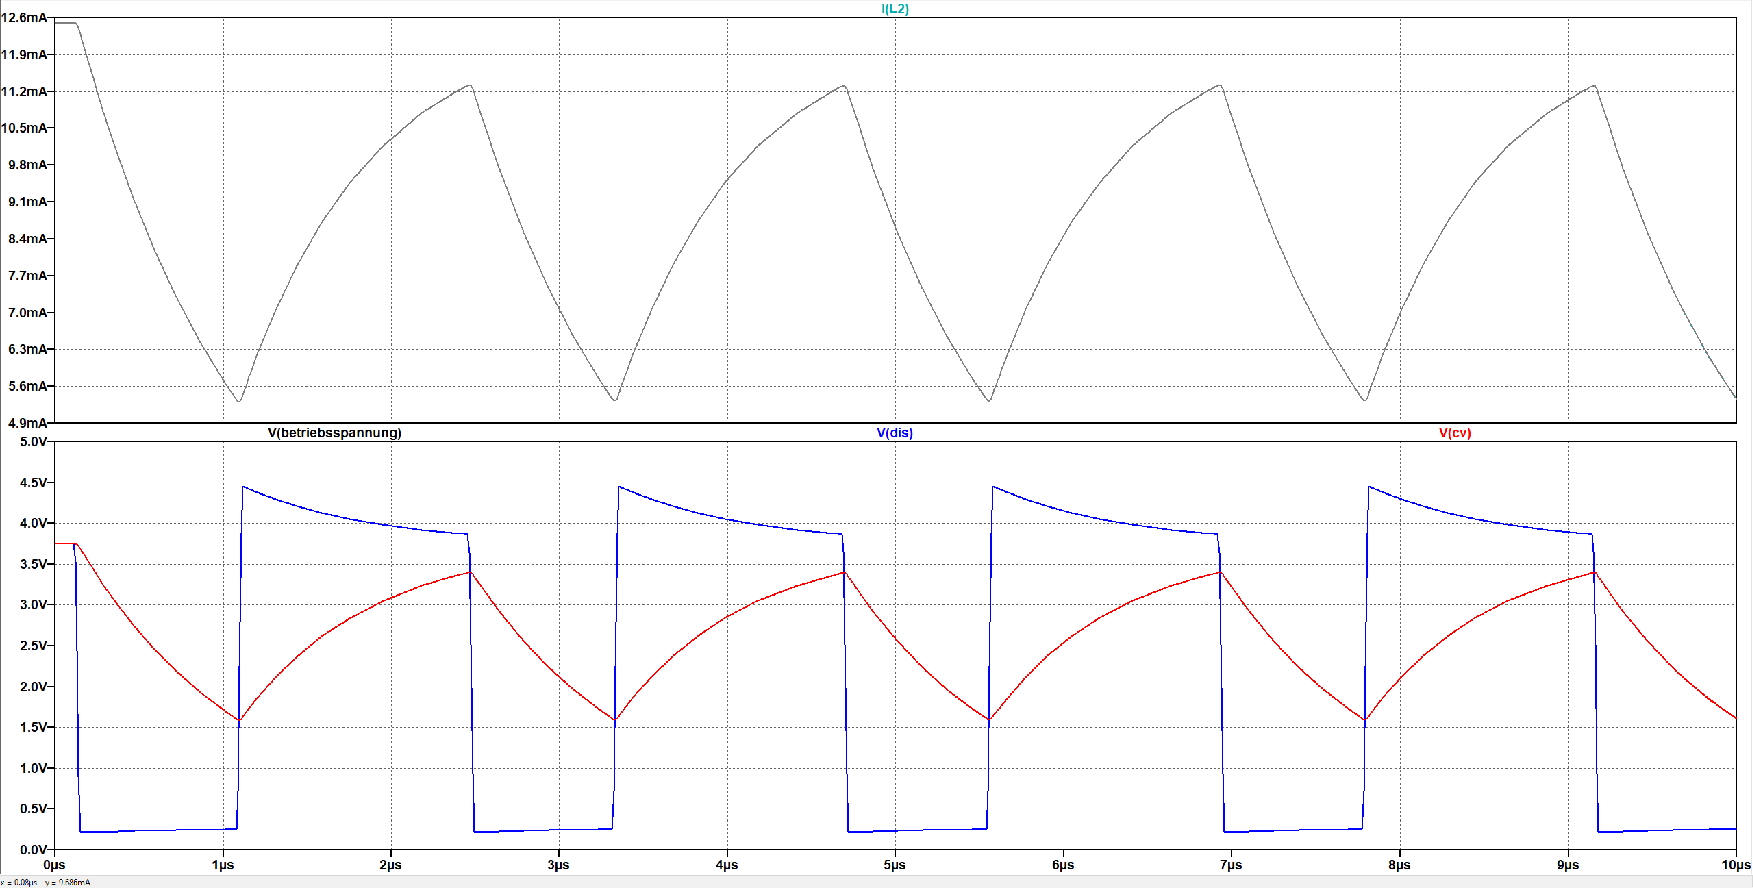
\includegraphics[width=1\linewidth]{fahrzeugerkennung/RL_Oszillator_ZB.png}
    \caption{RL-Oszillator mit NE555 Zeitsignale}
\end{figure}

Im oberen Diagramm ist der Verlauf des Stromes durch die Spule zu erkennen der wie erwartet zu- und abnimmt. Im unteren Diagramm ist in 
schwarz die Betriebsspannung als Referenz in rot der CV Pin und in blau der DIS Pin des NE555. Das rote Signal wechselt zwischen zwei drittel der Betriebsspannung 
und einem drittel der Betriebsspannung mit einer Frequenz von $f = \SI{438}{\kilo\hertz}$ bei einer Induktivität von $L = \SI{300}{\micro\henry}$, einem Widerstand $R4 = 100\Omega$ und einem
Widerstand $R5 = 300\Omega$. Die Simulation entspricht hier der Theorie, jedoch bricht das blaue Signal am PIN DIS in der Einschaltphase ein.
Der grund dafür ist der interne Widerstand des NE555, der ab einem gewissen Stromverbrauch für einen Spannungsabfall sorgt. Da es meist besser ist mit
niedrigen Frequenzen zu arbeiten ist es nach den Gleichungen \ref{eq:i_L} und \ref{eq:tau_RL} entweder nötig die Induktivität zu erhöhen oder die Widerstände zu verkleinern.
Die Induktivität lässt sich aber entweder durch erhöhen der Windungen oder durch Vergrößerung der Spule erreichen, was in vielen Fällen nicht möglich ist oder zunehmends kostspielig ist.
Die Reduktion der Widerstände führt zu einer Zunahme des Stromes und der Verlustleistung, was auch unerwünscht ist.
Aus diesen Gründen ist der RL-Oszillator nur für hohe Frequenzen geeignet. In der nächsten Abbildung sieht man die Schaltung bei verschiedene Induktivität
nämlich bei $L2 = \SI{100}{\micro\henry}$ und bei $L2 = \SI{1}{\milli\henry}$

\begin{figure}[H]
    \centering
    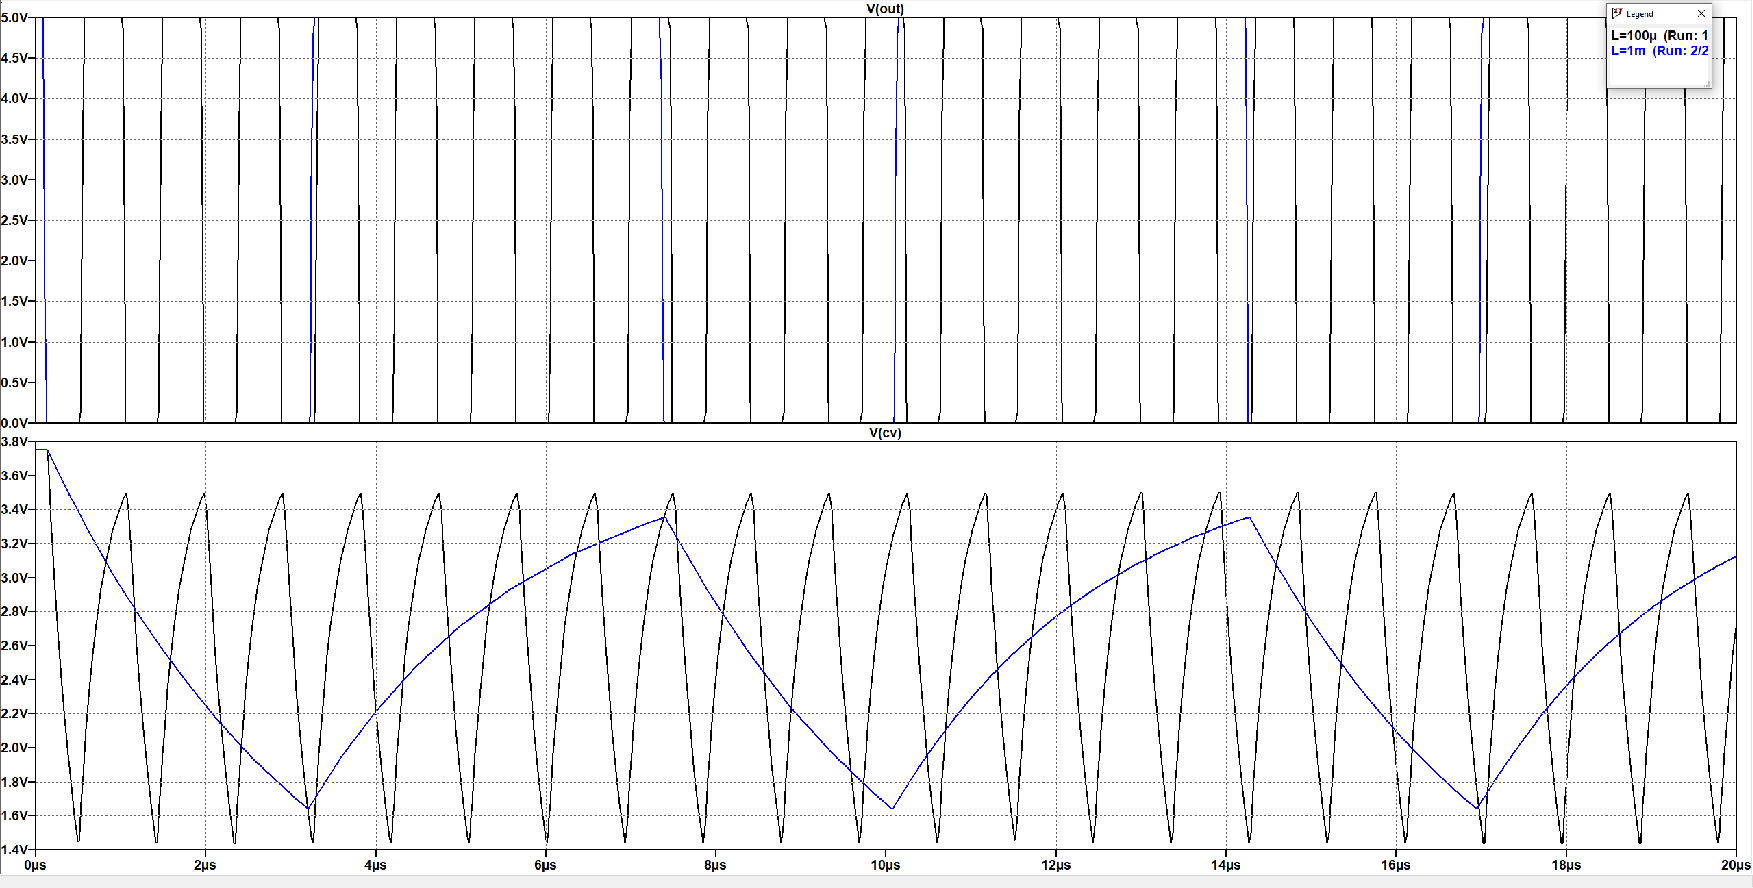
\includegraphics[width=1\linewidth]{fahrzeugerkennung/RL_Oszillator_vergleich2_ZB.png}
    \caption{Vergleich des NE555-Oszillators bei unterschiedlichen L}
\end{figure}

Eine Verzehnfachung der Induktivität führt zu einer Reduktion der Oszillatorfrequenz um den Faktor 10.

\begin{equation} \label{iq:f_NE555}
    f \propto \frac{1}{L}
\end{equation} 

\pagebreak
\subsubsection{Messung paramagnetischer Metalle}
Da nicht alle Metalle ferromagnetische Eigenschaften haben werden viele Stoffe wie Aluminium. Kupfer oder diverse Legierungen
von einer niederfrequenten Messung der Induktivität nicht wahrgenommen. Ein Effekt, welcher bei elektrischen Leitern abhilfe schaffen kann, sind 
die Eddy Currents. Wenn in einem Leiter ein magnetischen Feld einwirkt erzeugt dieses im Objekt Ströme, die wiederum ihr eigenes magnetische Feld erzeugen.
Die fließenden Ströme erzeugen im Objekt Ohmsche Verluste, welche normalerweise unerwünscht sind. Sie wirken auch einer Änderung der magnetischen Feldes entgegen,
da sie selbst Energie brauchen um ihre Richtung zu ändern. Je größer die Frequenz der eingespeisten Felddichte $B$ desto stärker wirkt die 
Flussdichte $B_{eddy}$ senkend auf die Gesamtflussdichte und so auf den magnetischen Fluss $\Phi$. 
Nach der Gleichung \ref{eq:L_phi} reduziert sich danach die Induktivität mit zunehmender Frequenz.


\begin{figure}[H]
    \centering
    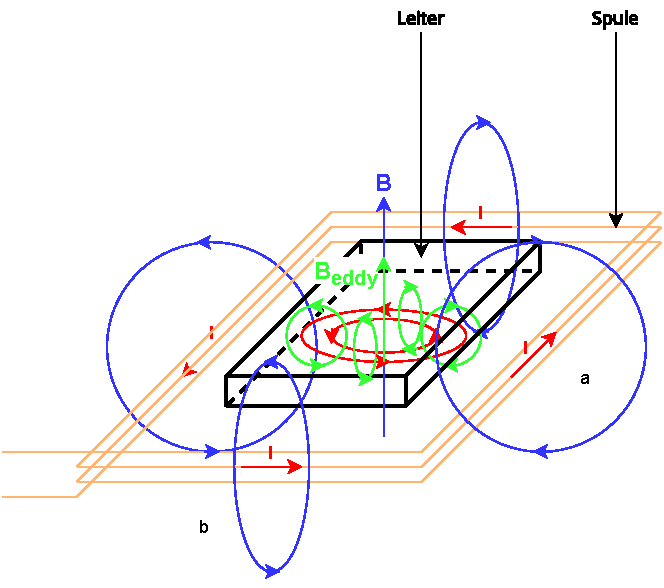
\includegraphics[width=0.6\linewidth]{fahrzeugerkennung/Eddy_Currents.pdf}
    \caption{Eddy Currents in einem Leiter}
\end{figure}

Bei sehr hohen Frequenzen ist jedoch zu beachten, dass der Skin-Effekt die Querschnittsfläche, durch die der Wechselstrom fließen kann,
reduziert. Somit nimmt der Effekt der Eddy-Currents ab. Diese Phänomene werden jedoch nicht in dieser Arbeit behandelt, da sie außerhalb des Rahmens der 
Fahrzeugerkennung liegen. 

\paragraph{LC Oszillatoren}\mbox{}\\

Im Vergleich zum RL-Oszillator, der über eine astabile Kippstufe lauft, kann ein LC Oszillator seine Resonanzfrequenz nur durch das verstellen der Induktivität und der Kapazität 
eines Kondensators verändern. Zudem gibt es in der Theorie keine Wirkverluste, da die Energie abwechselnd zwischen magnetischer und elektroscher Energie umgewandelt wird. In der Realität gibt es jedoch
ohmsche Verluste, die zu einem Abklingen der Schwingung führen. Es braucht daher ein aktives Glied wie ein Transistor oder ein Operationsverstärker, der den Oszillator mit Energie versorgt.
\\
Der zeitliche Verlauf einer ungedämpften Schwingung kann in LTSPice simuliert werden indem wir eine Sprungfunktion auf ein LC Glied geben und einen Widerstand in Serie zum Kondensator oder zur
Spule geben.

\begin{figure}[H]
    \centering
    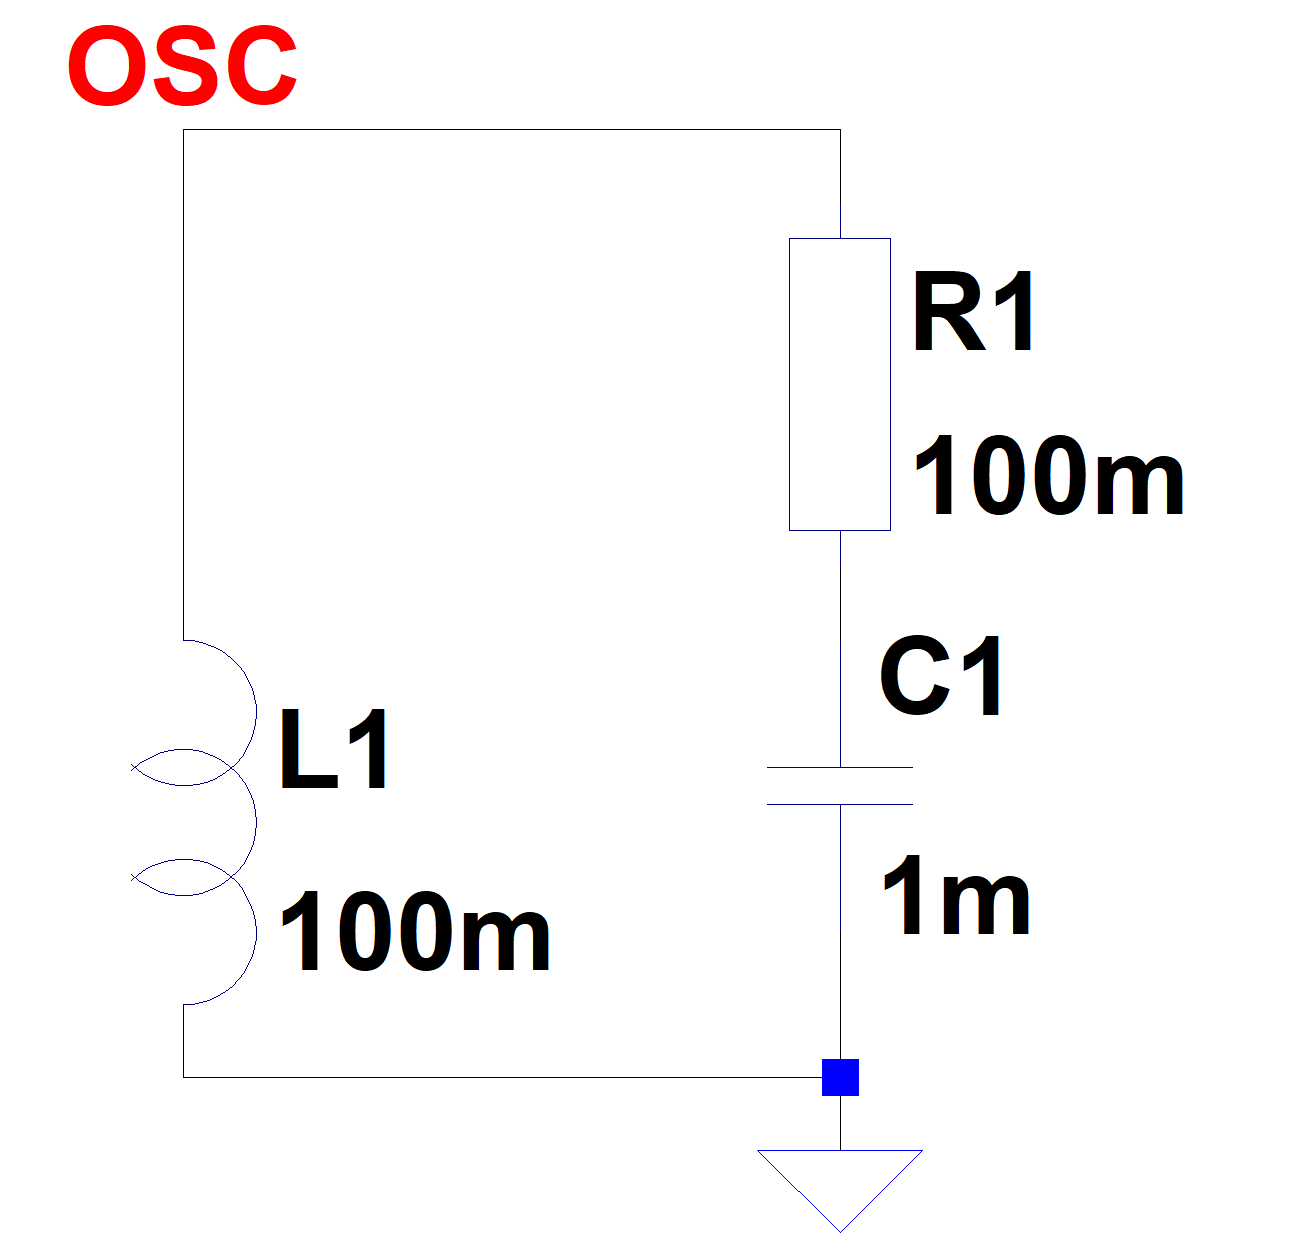
\includegraphics[width=0.6\linewidth]{fahrzeugerkennung/LC_Parallel.PNG}
    \caption{Parallelschwingkreis in LTSpice}
\end{figure}

\begin{figure}[H]
    \centering
    \includegraphics[width=1\linewidth]{fahrzeugerkennung/gedämpfte_schw.PNG}
    \caption{Gedämpfte Schwingung}
\end{figure}

Aus der Simulation ergibt sich über eine Cursormessung für die angegebenen Werte $L = \SI{100}{\milli\henry}$ und $C = \SI{100}{\milli\farad}$ eine Resonanzfrequenz einen Wert von $f = 15.85Hz$. Die Resonanzfrequenz für einfache LC-Schwingkreise lässt sich mit der
Thomsonschen Schwingungsgleichung errechnen:

\begin{equation} \label{eq:thomson}
    f = \frac{1}{2 \cdot \pi \sqrt{L \cdot C}}
\end{equation}

Wobei \\
$f$ = Resonanzfrequenz des LC-Gliedes\\
$L$ = Induktivität der Spule\\
$C$ = Kapazität des Kondensators\\

Wenn man die Werte $L = \SI{100}{\milli\henry}$ und $C = \SI{100}{\milli\farad}$ ind die Gleichung \ref{eq:thomson} einsetzt erhält man eine Resonanzfrequenz von $f = 15.915Hz$.
Allgemein tritt in LC-Glieder bei einer Phasenlage von $\varphi_{LC} = 180^{\circ}$ und bei der Frequenz nach der Thomsonschen Gleichung \ref{eq:thomson}  Resonanz auf. 

\paragraph{Einfluss von Induktivitätsänderungen auf LC-Oszillatoren}\mbox{}\\

Für die Fahrzeugerkennung ist es von Relevanz zu wissen wie die Frequenz dieser Oszillatoren auf die Änderung der Induktivität der im Boden verbauten Spule reagiert.
Wenn eine Parklücke frei ist besitzt die Spule eine Induktivität von $L_{0}$ und hat nach der Thomsonschen Gleichung \ref{eq:thomson} eine Resonanzfrequenz $f_{0}$. Für kleine Änderungen $\Delta L$ kann eine Näherung
der Frequenzänderung gemacht werden indem man in den Punkt $(f_{0}, L_{0})$ in den Graphen der Thomsonschen Gleichung aufgetragen über die Induktivität $L$ eine Tangente in diesen Punkt legt. Bei einer 
Kapazität von $C = \SI{1}{\micro\farad}$ erhält man folgenden Graphen: 

\begin{center}
    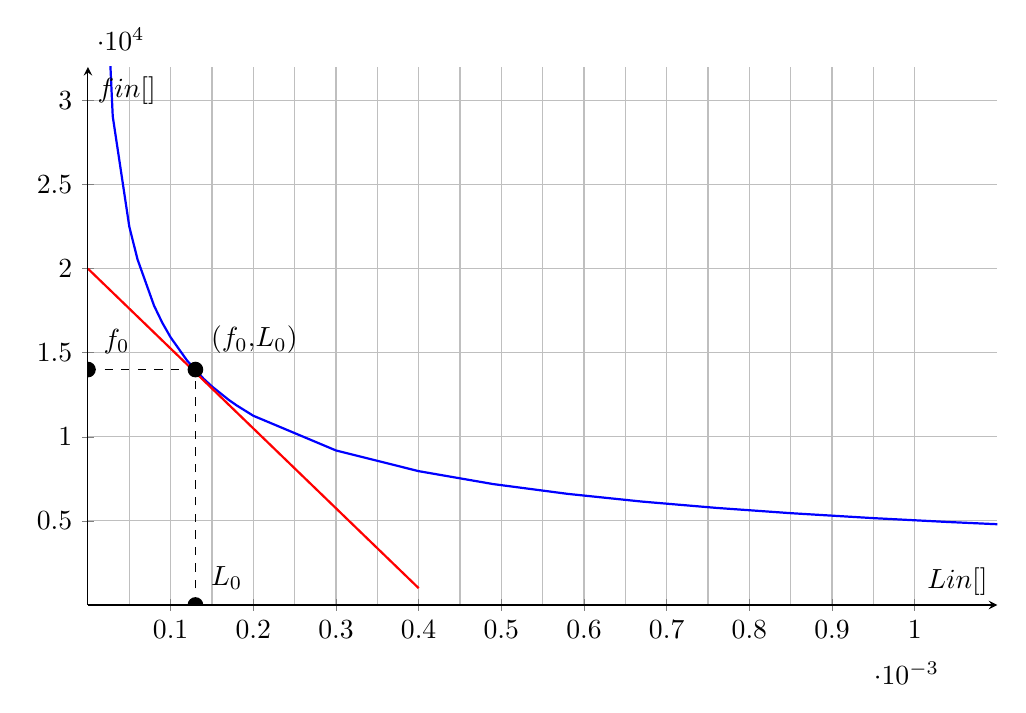
\begin{tikzpicture}
        
        \begin{axis}[
                axis x line=middle, 
                axis y line=middle, 
                xlabel={$L \text{ in } \si[]{\henry}$}, 
                ylabel={$f \text{ in } \si[]{\hertz}$}, 
                x=15cm/0.001,    
                y=0.0003cm,    
                grid =both,
                minor x tick num=1,
                subtickwidth=0pt,
                xtick={0,0.0001,...,0.001}, 
                ytick={0,5000,...,30000}, 
                xmin=0,  
                xmax=0.0011,   
                ymin=0,  
                ymax=32000,  
                scale = 0.7 
        ]
        
        \addplot [blue, thick, samples at={0,0.000001,0.000005,0.00001,...,0.0002,0.0003,0.0004,...,0.002}] {1/(2*pi*sqrt(x*1e-6))};
        \addplot[mark=none, red, thick] coordinates {(0, 20000) (0.4e-3, 0.1e4)};
        \addplot[mark=none, black, dashed] coordinates {(0, 1.4e4) (0.13e-3, 1.4e4)};
        \addplot[mark=none, black, dashed] coordinates {(0.13e-3, 0) (0.13e-3, 1.4e4)};
        \node[label={45:{($f_{0}$,$L_{0}$)}},circle,fill,inner sep=2pt] at (axis cs:0.13e-3,1.4e4) {};
        \node[label={45:{$L_{0}$}},circle,fill,inner sep=2pt] at (axis cs:0.13e-3,0) {};
        \node[label={45:{$f_{0}$}},circle,fill,inner sep=2pt] at (axis cs:0,1.4e4) {};
    \end{axis}
    \end{tikzpicture}
\end{center}

Mit dieser Näherung kann man mit des Differentials der Thomsonschen Gleichung \ref{eq:thomson} die Änderung des Funktionswertes $f(L \pm \Delta L) = \Delta f \approx df$ 

\paragraph{Messung der Frequenz eines Colpitts-Oszillator}\mbox{}\\

Der Colpitts-Oszillator ist eine Variante des LC-Oszillator und wird in der Praxis oft mit einem aktiven Element betrieben. Im Vergleich zu einem einfachen LC-Glied besitzt dieser Oszillator
zwei Kondensatoren. Das Schaltbild sieht so aus:

\begin{figure}[H]
    \centering
    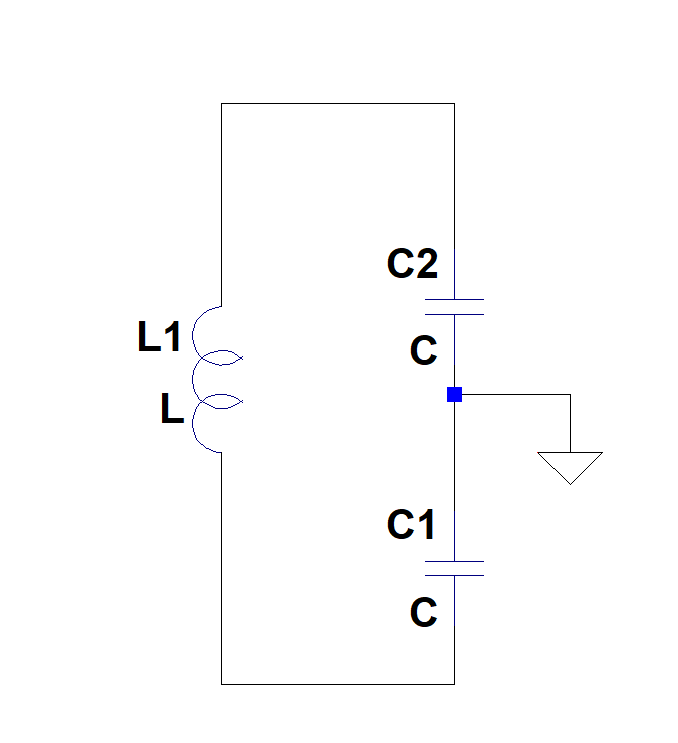
\includegraphics[width=0.4\linewidth]{fahrzeugerkennung/Colpitts_LC.PNG}
    \caption{Colpitts LC-Glied}
\end{figure}

Dieses LC-Glied wird als Rückkoppelglied eingesetzt und sorgt für die nötige Phasendrehung von $\varphi_{LC} = 180^{\circ}$. Wie man in der obigen Abbildung sehen kann liegen die Kondensatoren 
$C_{1}$ und $C_{2}$ in Serie. Es ergibt sich daher eine Gesamtkapazität von $C_{ges}$.

\begin{equation} \label{eq:c_gescolpitts}
    C_{ges} = \frac{C_{1} \cdot C_{2}}{C_{1} + C_{2}}
\end{equation}
Durch einsetzen in die Thomsonsche Gleichung erhält man für die Resonanzfrequenz eines Colpitts-Oszillator:
\begin{equation} \label{eq:colpitts}
    f = \frac{1}{2 \cdot \pi \sqrt{L \cdot \left( \frac{C_{1} \cdot C_{2}}{C_{1} + C_{2}} \right) }}
\end{equation}

Wobei \\
$f$ = Resonanzfrequenz des Colpitts-Oszillator\\
$L$ = Induktivität der Spule\\
$C_{1}$ = Kapazität des Kondensators $C_{1}$\\
$C_{2}$ = Kapazität des Kondensators $C_{2}$\\

\pagebreak
Das aktive Element wird an die Anschlüsse der Spule angeschlossen muss selbst eine Phasendrehung von 180° liefern. Zusätzlich muss die Verstärkung des Gliedes größer als 1 damit eine dauerhafte 
Schwingung entstehen kann. Mit einem Operationsverstärker muss der nicht invertierende Eingang auf eine Bezugsspannung gelegt werden. Diese Bezugsspannung wird of in die Mitte des Versorgungsspannungsbereich
gelegt. Bei einem Spannungsbereich von $\SI{0}{\volt}$ bis $\SI{5}{\volt}$ ist eine Bezugsspannung von $\SI{2,5}{\volt}$ sinnvoll. Der invertierende Eingang wird an das Colpitts LC-Glied angeschlossen. Der Ausgang des Operationsverstärker wird über
einen Widerstand an das LC-Glied geschalten, damit das Rückkoppelglied besser vor übersteuerungen am Ausgang des Operationsverstärkers geschütz ist. 

\begin{figure}[H]
    \centering
    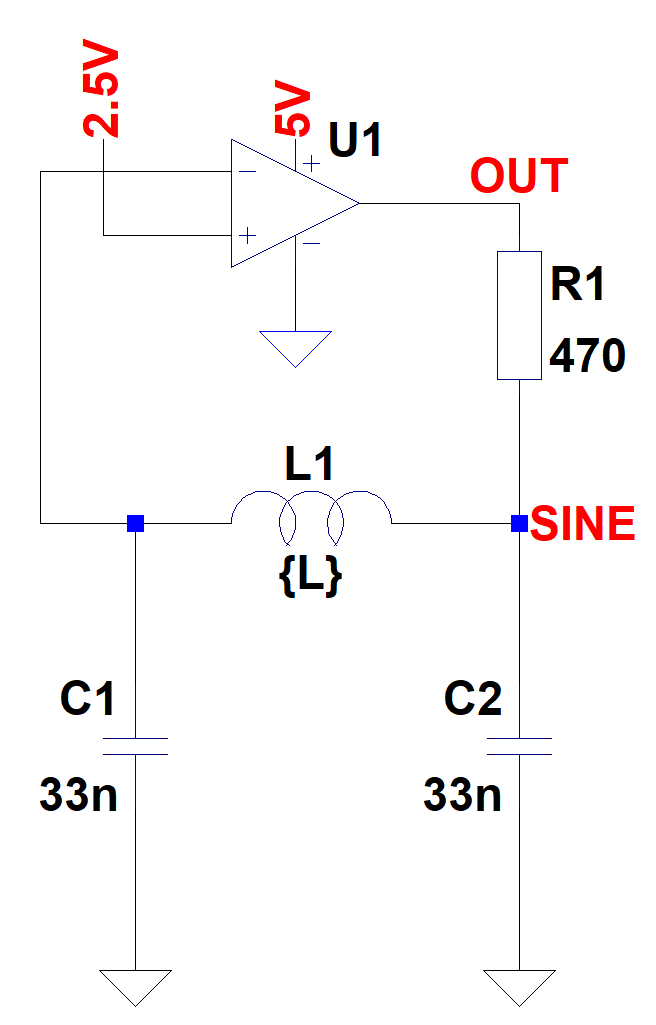
\includegraphics[width=0.4\linewidth]{fahrzeugerkennung/Colpitts_active.PNG}
    \caption{Aktiver Colpitts-Oszillator}
\end{figure}

Wenn man nun verschiedene Werte für Induktivität einsetzt ergibt sich durch die Simulation dieses Schaltbildes folgende Zeitsignale für den Ausgang des Operationsverstärker OUT und der Spannung SINE:

\begin{figure}[H]
    \centering
    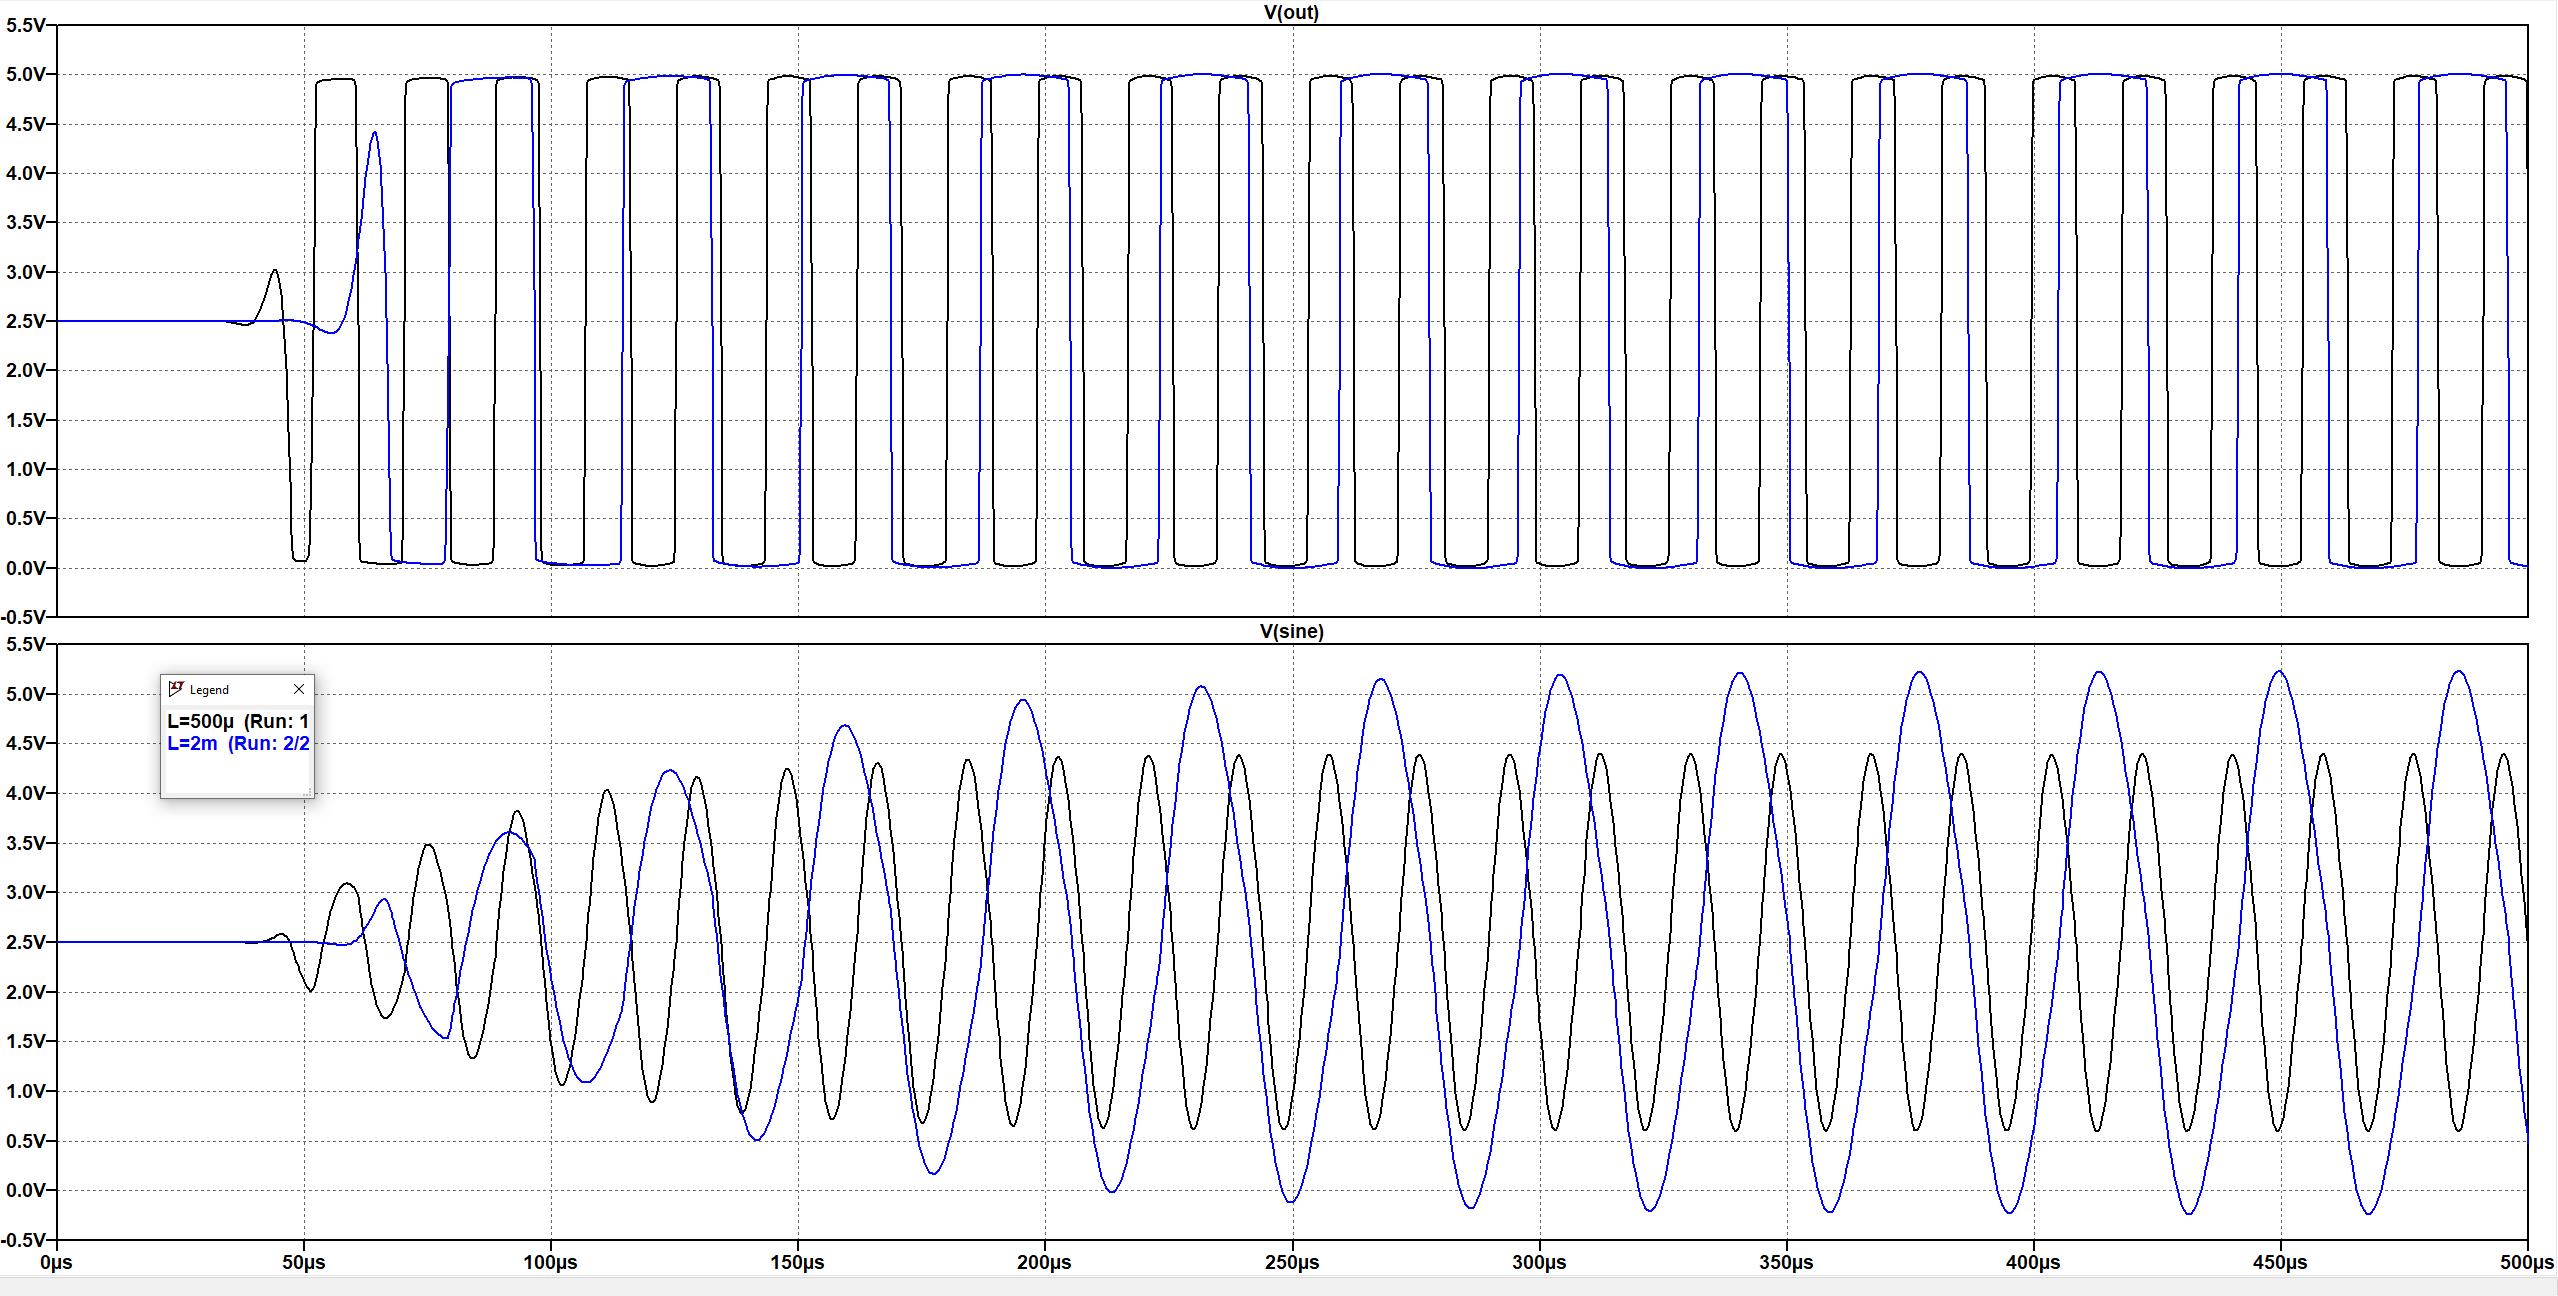
\includegraphics[width=1\linewidth]{fahrzeugerkennung/Colpitts_active_ZB.PNG}
    \caption{Zeitsignale Colpitts-Oszillator}
\end{figure}


\subsection{RS485 Bussystem}
\subsubsection{Überblick}
\subsubsection{Elektrische Spezifikation}
\subsubsection{Implementation eines eigenen Protokolls}

\subsection{Mikrokontroller Slave-Geräte}
\subsubsection{Überblick}
\subsubsection{Atmega328PB}
\subsubsection{Peripherie des Mikrokontrollers}
\paragraph{Spannungswandler}
\paragraph{RS485 Pegelwandler}
\paragraph{Digitale Ein- und Ausgänge}
\subsubsection{Layout des Slave-Gerätes}
\subsubsection{Gehäuse}


\subsection{USB-Master}
\subsubsection{USB-Bussadapter Gerät}
\paragraph{Überblick}
\paragraph{FT232RL}
\paragraph{Spannungsversorgung}
\paragraph{USB-C Anschluss}
\paragraph{Layout des Master-Geräts}
\paragraph{Gehäuse}

\subsubsection{Master Programm}
\paragraph{Benötigte Software}
\paragraph{Adressvergabe}
\paragraph{Frequenzauslesung}

\paragraph{Auswertung}
\paragraph{API-Post}

\subsubsection{RaspberryPi als Mastergerät}
\paragraph{SSH Remote Zugriff}
\paragraph{Code Deployment}
\paragraph{Unittest}

\pagebreak


